\documentclass[crop=false]{standalone}
\usepackage{graphicx}
\graphicspath{{images/}}
\usepackage{blindtext}
\usepackage[immediate]{silence}
\WarningFilter[temp]{latex}{Command}
\usepackage{sectsty}
\DeactivateWarningFilters[temp]
\usepackage{array}
\usepackage{enumerate}
\usepackage{graphicx}
\usepackage{listings}
\usepackage{color}
\usepackage{setspace}
\usepackage[margin=1in]{geometry}
\usepackage{mathtools}
\usepackage{wrapfig}
\usepackage{titlesec, titleps}
\usepackage{longtable}
\usepackage{booktabs}
\usepackage{multirow}
\usepackage{multicol}
\usepackage{pdflscape}
\usepackage{float}
\usepackage{subcaption}
\usepackage{lscape}
\usepackage[hidelinks]{hyperref}
\hypersetup{
    colorlinks,
    citecolor=black,
    filecolor=black,
    linkcolor=black,
    urlcolor=black
}


\sectionfont{\centering}


\begin{document}
\pagenumbering{gobble}
    

    \newpage
    \newpage
    \pagenumbering{arabic}
        
    \clearpage
\subsection{Mixed Range Radio Board}
    \subsubsection{Design}
        The objective of the M2RB is to facilitate both long and short range communication. The long-range communication is handled by a Spartan 7 FPGA and a custom RF front end to achieve a high speed connection to the ground station. The short-range communication is handled by an nRF52832 running Bluetooth Mesh.
        \begin{figure}[H]
            \centering
            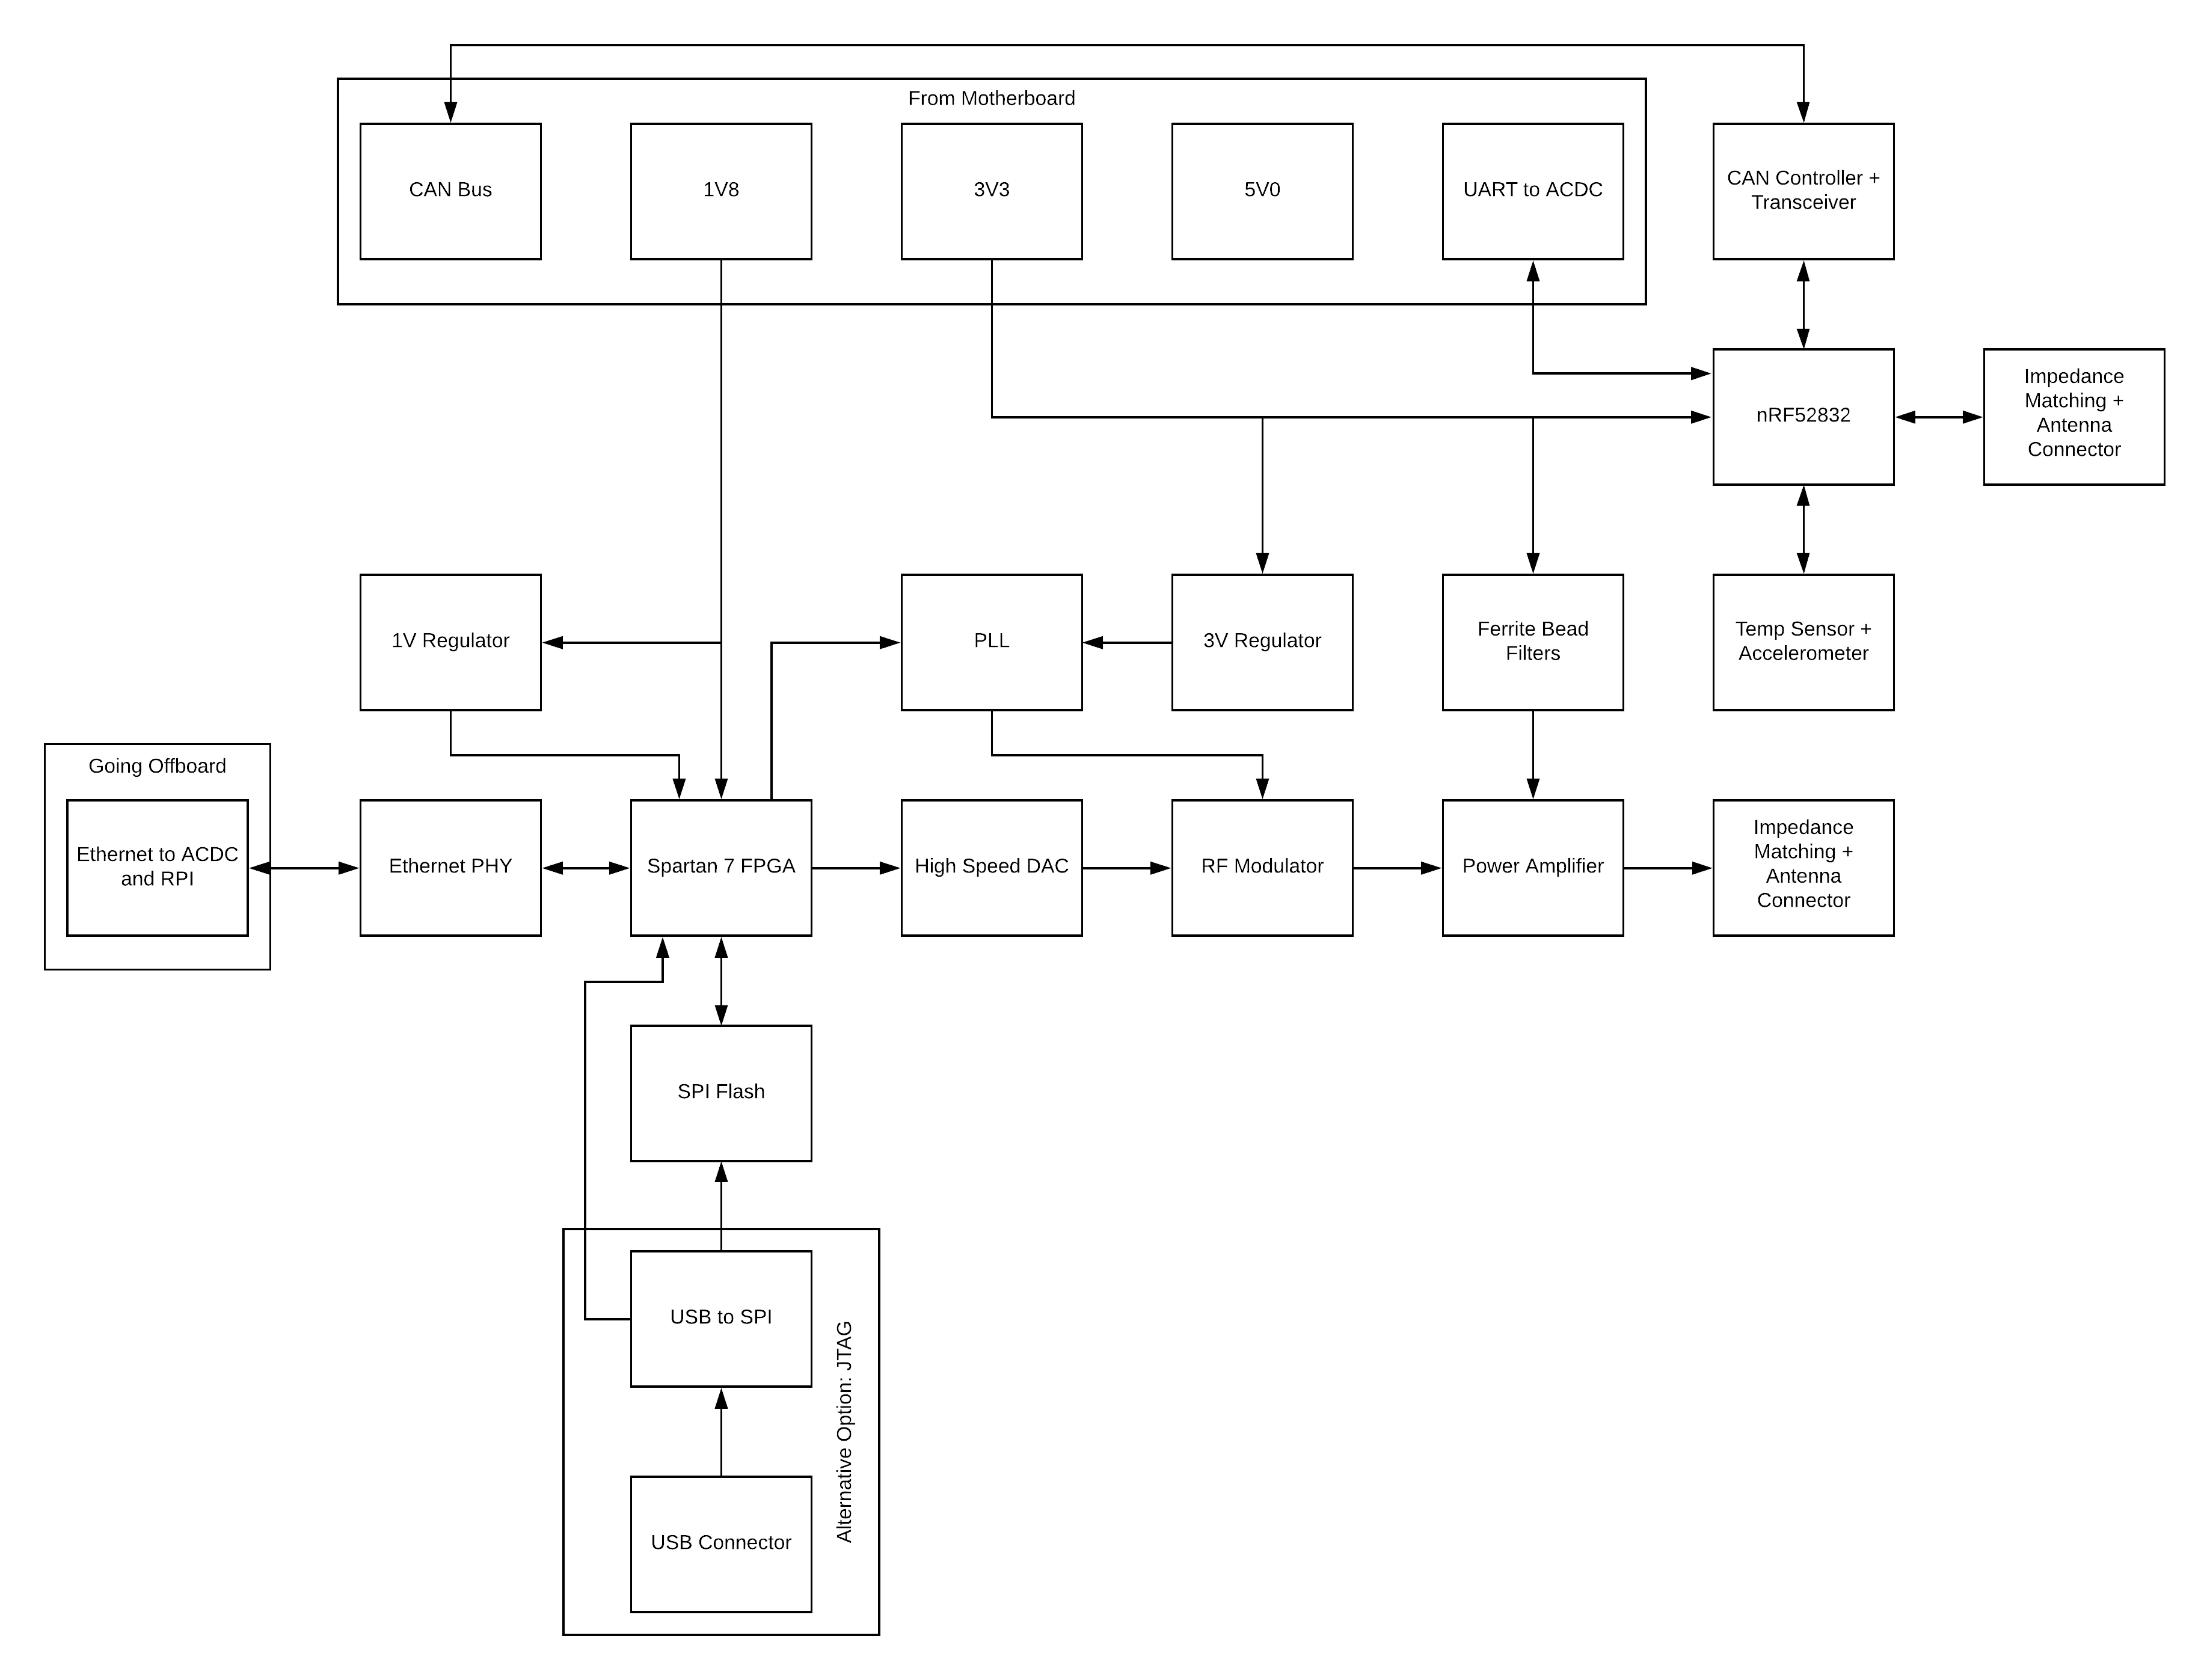
\includegraphics[width=\textwidth]{M2RB Hardware Diagram.PNG}
            \caption{M2RB Hardware Flow Chart}
            \label{fig:M2RBHardwareDesign}
        \end{figure}
            
        The nRF52 was chosen for short-range communication due to both its feature set and ease of implementation. The relatively high transmit power (4dBm) and the extremely good receiver sensitivity (-89dBm at 2Mbps) make the nRF52 an exceptional choice for reliability. This is an extremely important characteristic since one of the short range connections is to the ABC. A poor connection could result in malfunction of the airbrake system, potentially causing an accident, up to a CATO.
            
        The nRF52 is being used instead of an older, but cheaper, 51 series due to the software development kit. Support for 51 series ended before official support for Segger Embedded Studio, which resulted in numerous problems in the 2019-20 year when developing software for an nRF 51 series SoC.
            
        The nRF52 was chosen over other 52 series SoCs primarily due to cost. The nRF52 is not performing any heavy computations. As a result, any device that supports Bluetooth Mesh at 2Mbps almost immediately meets all requirements.
        
        \begin{figure}[H]
            \centering
            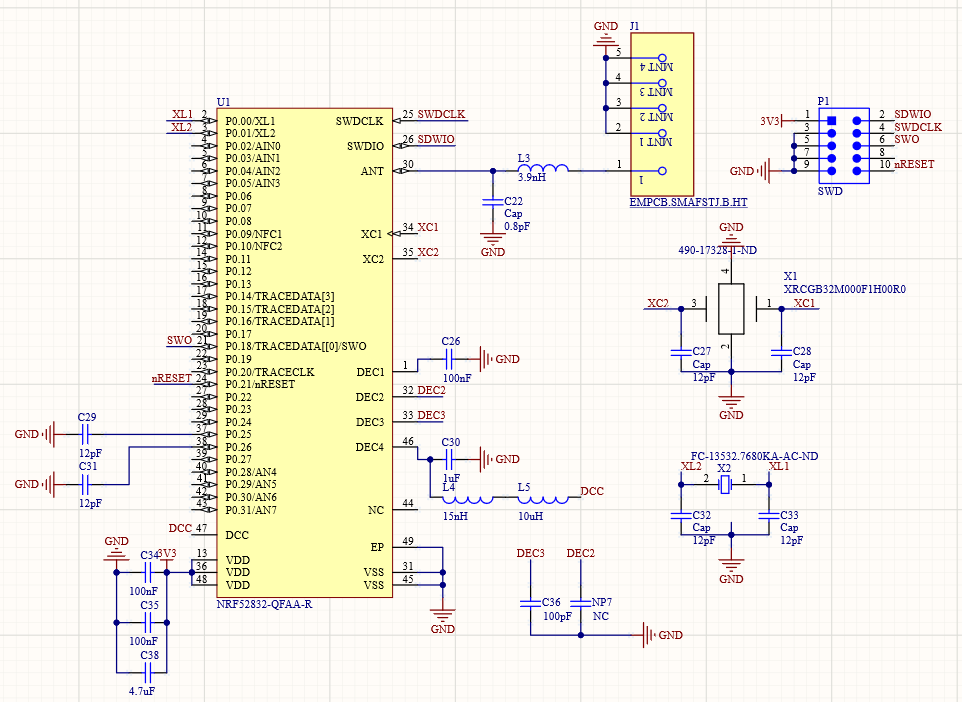
\includegraphics[width=\textwidth]{M2RBnRF.PNG}
            \caption{nRF52832 Schematic}
            \label{fig:M2RBnRF52}
        \end{figure}
            
        Figure \ref{fig:M2RBnRF52} shows the schematic for the nRF52 used on the M2RB. Everything shown is based off of the typical applications schematic using the internal switched mode power supply. There are a number of I/O which are not displayed on the schematic. This is because almost all of the I/O pins on the nRF52 are interchangeable, so the exact pins that will be used will be determined during PCB routing to simplify the routing as much as possible.
        
        \begin{figure}[H]
            \centering
            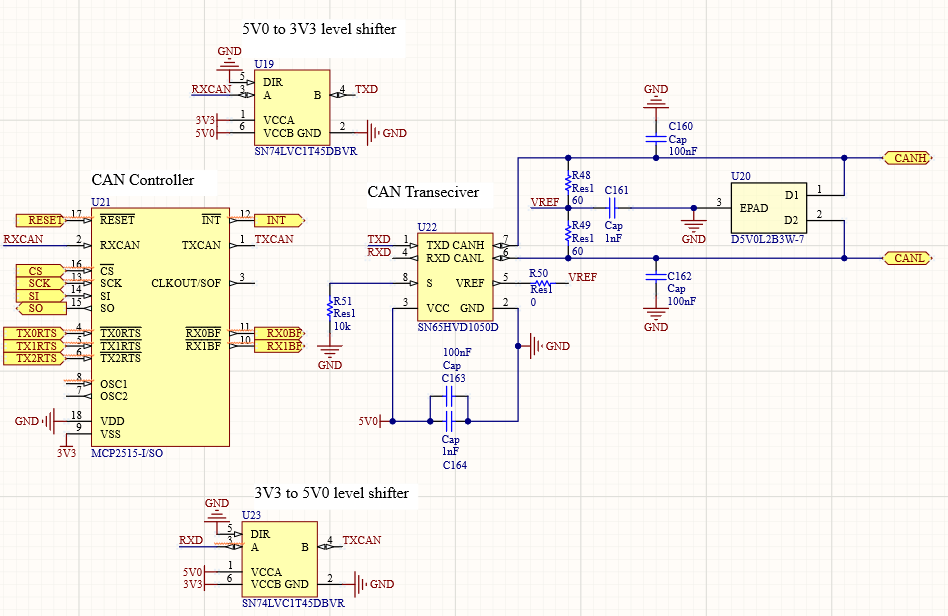
\includegraphics[width=\textwidth]{M2RBCAN.PNG}
            \caption{CAN Schematic}
            \label{fig:M2RBCAN}
        \end{figure}
            
        \begin{wrapfigure}{R}{0.5\textwidth}
            \centering
            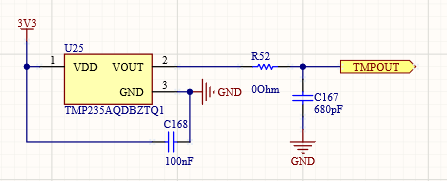
\includegraphics[width=0.48\textwidth]{M2RBTemp.PNG}
            \caption{The temperature sensor used by the nRF52}
            \label{fig:M2RBTemp}
            \smallskip\par
            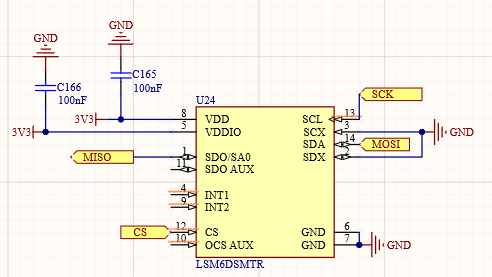
\includegraphics[width=0.48\textwidth]{M2RBAccel.PNG}
            \caption{The accelerometer used by the nRF52}
            \label{fig:M2RBAccel}
        \end{wrapfigure}
            
        Figure \ref{fig:M2RBCAN} shows the CAN controller and transceiver schematic used by the nRF52. The CAN controller communicates with the nRF52 using a mixture of SPI and an interrupt along with some registers. The controller then communicates with the transceiver by using level shifters to convert voltages between the 3.3V controller to the 5V CAN transceiver. The CAN transceiver also features a set of zener diodes for ESD protection.
            
        The nRF52 is also gathering data from a couple sensors, seen in figures \ref{fig:M2RBTemp} and \ref{fig:M2RBAccel}. Figure \ref{fig:M2RBTemp} is just an analog temperature sensor. Every board has one in order to monitor the temperature throughout the Flight Computer in order to determine how hot the electronics get during launch for future reference. Figure \ref{fig:M2RBAccel} is a basic accelerometer. This accelerometer has no correction for gravity, or any other sensors on it, so it is just measuring the acceleration applied to each axis of the PCB. This is what is wanted, since the main use of this accelerometer is to determine how much vibration there is during launch. This accelerometer can communicate via SPI or I2C. Since it is in SPI mode, some pin names do not fully match.
        
        \pagebreak
         
        The long range portion of the M2RB is based around a custom RF front end. This front end is transmit only and consists of a PLL, DAC, and modulator. The PLL can be controlled in software to tune anywhere in the 900MHz band. The DAC has 14 bits of resolution and contains both an I and Q channel integrated into one device. The modulator is designed to work with the chosen DAC which greatly simplifies design.
            
        The RF front end requires an FPGA to control it due to high data rate requirements. The FPGA acts as a baseband modulator and outputs its data to the DAC. The FPGA also controls the center frequency of the transmission through a digital interface with the PLL.
            
        The FPGA chosen for baseband modulation is a Xilinx Spartan 7. In order to gather data to send to ground the FPGA communicates using an Ethernet connection shared with the ACDC and Raspberry Pis.
            
        \begin{figure}[H]
            \centering
            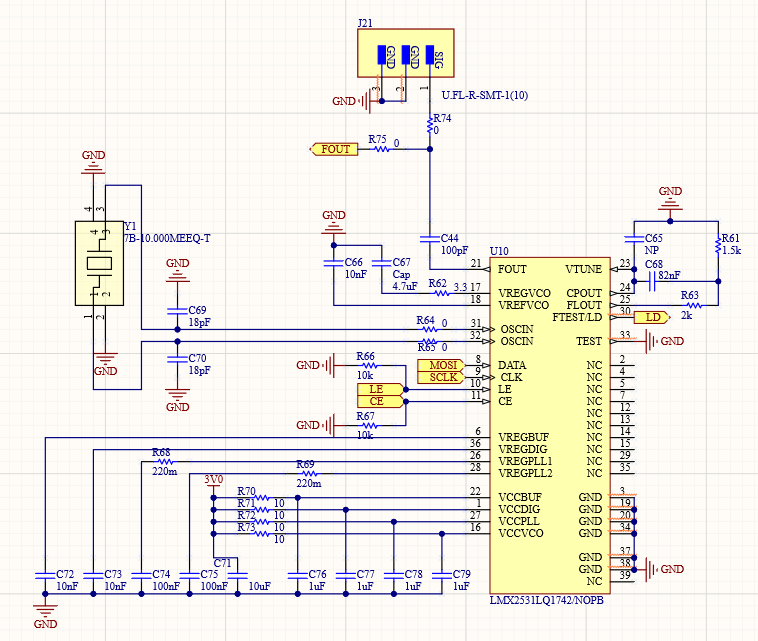
\includegraphics[width=\textwidth]{M2RBPLL.PNG}
            \caption{LMX2531LQ1742 PLL}
            \label{fig:M2RBPLL}
        \end{figure}
            
        In order to perform upconversion an n fractional PLL is being used to provide a local oscillator. Figure \ref{fig:M2RBPLL} shows the schematic for the LMX2531LQ1742. This PLL was chosen for two reasons. It has a built in VCO, which greatly simplifies design, and is also programmable via SPI using 1.8V logic. The 1.8V logic is important since that is the max voltage that the I/O of the FPGA can handle.
        
        The PLL uses a 10MHz reference oscillator in order to generate an output in the 900MHz ISM band. If the PLL is used in fractional mode, then the PLL can achieve <200kHz channel spacing which will allow for fine control of the center frequency. However, using the PLL in fractional mode can result in additional spurs, potentially resulting in transmissions outside the band of interest.
                
        \begin{wrapfigure}{R}{0.5\textwidth}
            \centering
            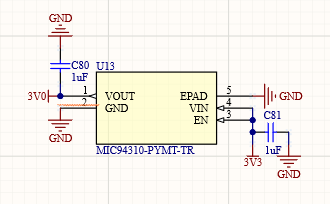
\includegraphics[width=0.48\textwidth]{M2RB3V.PNG}
            \caption{3V regulator for the PLL}
            \label{fig:M2RB3V}
            
            \smallskip\par
            
            \centering
            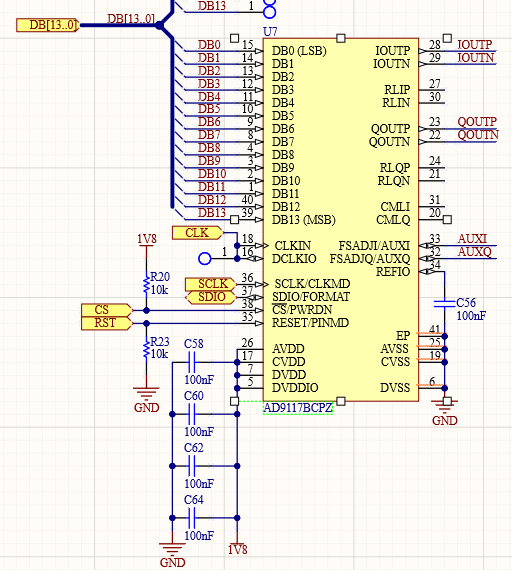
\includegraphics[width=0.48\textwidth]{M2RBDAC.PNG}
            \caption{High speed DAC}
            \label{fig:M2RBDAC}
        \end{wrapfigure}
        
        If the PLL is used in integer only mode, then the channel space will be approximately 500kHz, but there will be no additional spurs from the fractional component. Since there is no need for fine control of the center frequency it makes more sense to use the PLL in integer mode.
        
        A U.FL connector is included with a 0Ohm resistor so that the output of the PLL can be easily measured for debug purposes.
        
        This PLL also requires a 3V supply. In order to provide a low noise supply to the PLL a linear regulator was used to drop the 3.3V rail down to 3V. \ref{fig:M2RB3V} shows the regulator.
            
        \smallskip\smallskip\smallskip\smallskip\smallskip\smallskip\smallskip\smallskip
            
        In order to transmit data an analog baseband signal needs to be generated with a DAC. Figure \ref{fig:M2RBDAC} shows the schematic for the AD9117BCPZ DAC. This DAC was chosen specifically because it was designed to easily interface with the IQ modulator used in this signal chain. The DAC has differential I and Q outputs. Both of these outputs use a single 14 bit parallel bus and are interleaved with a 125MHz DDR clock. The DAC can also be programmed over SPI. This allows various clock settings to be configured and more importantly it allows two low speed auxillary DACs to be programmed. These DACs are useful since they can be adjusted to fix IQ imbalances in software.
        
        Although the DAC is capable of using up to a 125MHz clock, this design will be clocking it around 20MHz. This clock frequency was chosen because the original digital baseband signal will have a fundamental frequency of 2.5MHz and matlab simulations showed 8x oversampling and digital filtering to be adequate digital signal processing.
        
        In order to make debugging easier, test points were added to every data pin and the clock pin on the DAC.
        
        \pagebreak
        
        \begin{figure}[H]
            \centering
            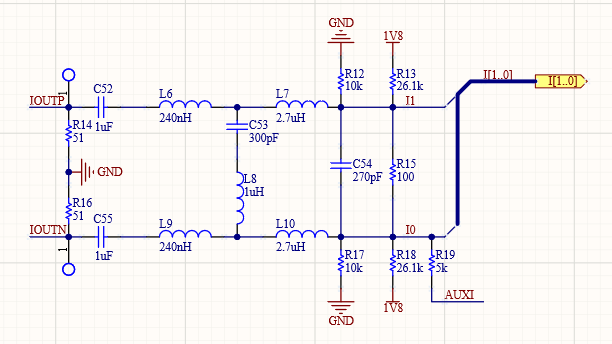
\includegraphics[width=\textwidth]{M2RBDACFilter.PNG}
            \caption{DAC Anti-imaging Filter}
            \label{fig:M2RBDACFilter}
        \end{figure}
        
        In order to reconstruct the intended analog signal an anti-imaging filter is required on the output of the DAC. Figure \ref{fig:M2RBDACFilter} shows the filter. The 51Ohm termination resistors are there because the DAC outputs current rather than voltage, so they are needed to generate a set voltage from the output current. The modulator that the DAC connects to requires a common mode bias of 500mV on its input. There are DC blocking capacitors on the input in order to AC couple the DAC output and a bias of 500mV is set using voltage dividers. There is a 100Ohm resistor on the output pins in order to limit the AC swing of the differential output to 2Vpp.
        
        \begin{figure}[H]
            \centering
            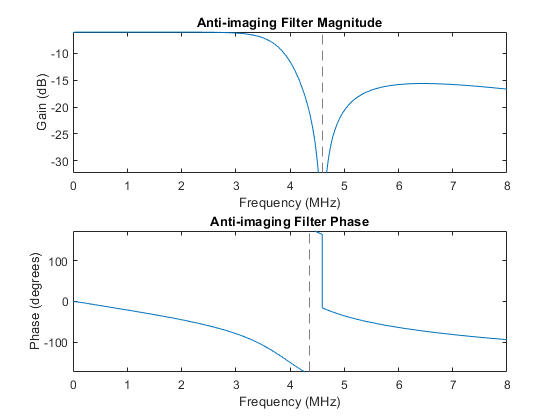
\includegraphics[width=\textwidth]{M2RBImagingFilter.png}
            \caption{DAC Anti-imaging Filter Frequency Response}
            \label{fig:M2RBFilterResponse}
        \end{figure}
        
        Figure \ref{fig:M2RBFilterResponse} shows the frequency response of the anti-imaging filter. A 3rd order elliptic filter with 0.1dB of passband ripple was chosen. The filter is designed to cut off before 5MHz, since that is the frequency of the second harmonic of the original signals fundamental frequency.
        
        Figure \ref{fig:M2RBFilterResponse} also shows the frequency response of the filter. The filter was designed to have an approximately linear phase up to 2.5MHz. This was done to keep a constant group delay in order to prevent distortion.
        
        \newpage
        
        \begin{figure}[H]
            \centering
            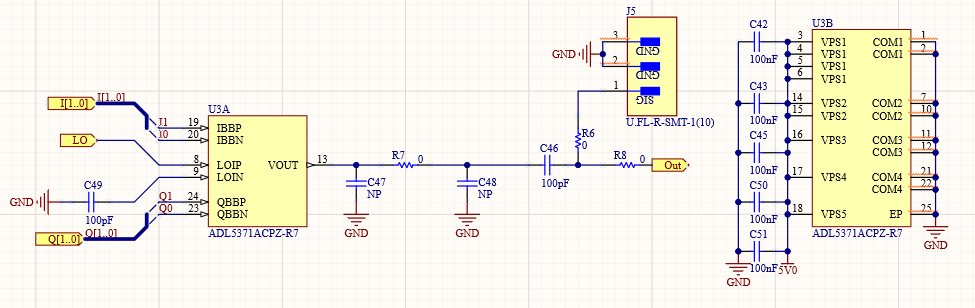
\includegraphics[width=\textwidth]{M2RBIQMod.PNG}
            \caption{IQ Modulator}
            \label{fig:M2RBIQMod}
        \end{figure}
        
        Figure \ref{fig:M2RBIQMod} shows the IQ modulator used to upconvert the DAC output. The modulator accepts two differential inputs for the IQ channels, which are provided by the DAC. The local oscillator negative pin is AC coupled to ground since the PLL is single ended instead of differential. The footprint for a simple LC filter is left on the output of the modulator. This is to allow an additional filter to remove out of band spurs and because the modulator output is not perfectly matched to 50 Ohms. The signal is then AC coupled to remove any DC bias from the modulator and it can be connected to the power amplifier or to a U.FL connector for probing.
            
        \begin{figure}[H]
            \centering
            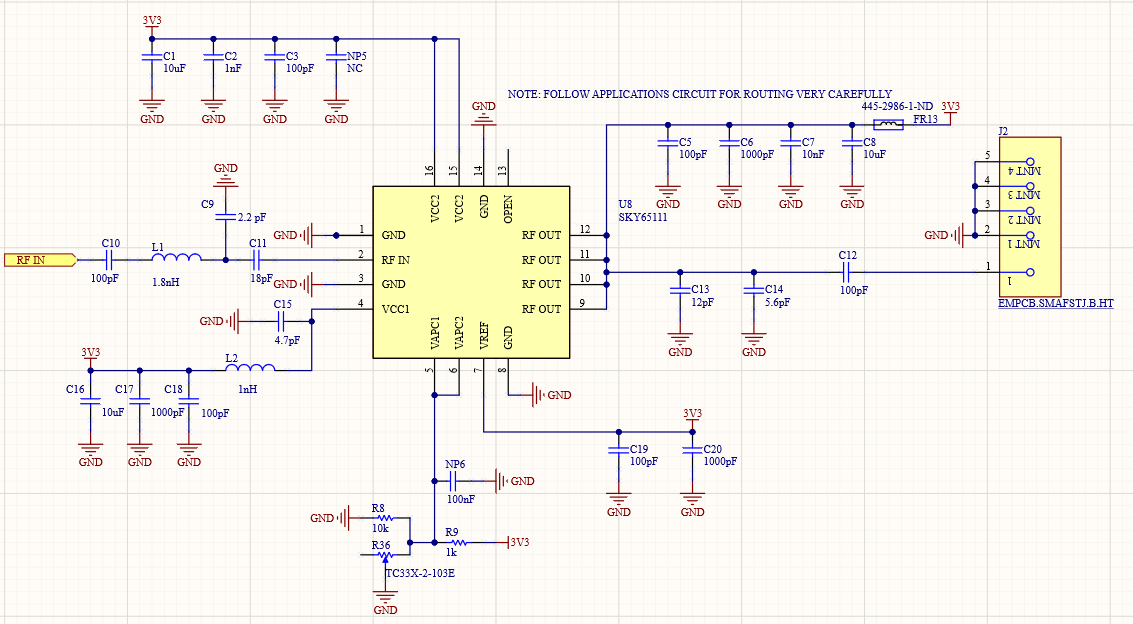
\includegraphics[width=\textwidth]{LMSPowerAmp.PNG}
            \caption{Power Amplifier}
            \label{fig:LMSPowerAmp}
        \end{figure}
            
        Figure \ref{fig:LMSPowerAmp} shows the schematic for power amplifier. It operates between 600MHz and 1100MHz. The amplifier features high linearity, with its P1dB appearing at about 29dBm output power. However, depending on the required amplifier gain the P1dB can appear at a higher power, such as 31dBm. Given that our most likely signal modulation method is 16QAM, which has a PAPR of about 2.5dB, a maximum average power of around 27dBm can be achieved without serious linearity problems. At this output power with a frequency in the 900MHz ISM band the power amplifier has an efficiency of around 25\%.
            
        \begin{wraptable}{R}{0.5\textwidth}
        %\begin{table}
        %\begin{center}
        \begin{tabular}{|c|c|c|}
        \hline
                        & 2Mbps                  & 20Mbps                 \\ \hline
        Frequency       & 915MHz                 & 915MHz                 \\ \hline
        Distance        & 8 km                   & 8km                    \\ \hline
        FSPL            & 109.7dB                & 109.7dB                \\ \hline
        BER             & \(10^{-6}\)            & \(10^{-7}\)            \\ \hline
        SNR             & 10dB                   & 15dB                   \\ \hline
        Thermal Noise   & -113.2dBm              & -106.2dBm              \\ \hline
        Rx Sensitivity  & -93.4dBm               & -83.4dBm               \\ \hline
        Transmit Power  & 27dBm                  & 27dBm                  \\ \hline
        Tx Antenna Gain & 0dB                    & 0dB                    \\ \hline
        Rx Antenna Gain & 0dB                    & 0dB                    \\ \hline
        Received Power  & -82.7dBm               & -82.7dBm               \\ \hline
        Fade Margin     & 10.7dBm                & 0.7dBm                 \\ \hline
        \end{tabular}
        \caption{Link Budget Information}
        \label{table:M2RBLink}
        %\end{center}
        %\end{table}
        \end{wraptable}
        
        Table \ref{table:M2RBLink} shows all of the information used in the link budget calculations for the long range portion of the M2RB. There are two cases presented, one capable of up to 2Mbps and the other capable of up to 20Mbps. The 2Mbps option utilizes a 1MHz wide QPSK encoding scheme. The 20Mbps option utilizes a 5MHz wide 16QAM encoding scheme.
            
        The 8km distance was chosen as the absolute max distance the rocket could get from the ground station. It will likely not get that far, and even if it does it will only result in a brief loss of data before the rocket would have landed anyways. As a result, this is a fairly conservative link budget.
            
        The expected data rate for a 720p 30fps video encoded with H.264 is approximately 13Mbps. As a result, 2Mbps will provide us with a significantly lower quality video, and 20Mbps has a significant amount of extra room for error if the H.264 encoding is not as efficient as expected. A lower BER was chosen for the 20Mbps option since its higher data rate meant that for the same BER there would be more errors per second and errors per frame of video.

        The thermal noise calculations assume a temperature of approximately 350k. While the interior of the rocket may get hotter than this, it provides a significant margin for heating on the ground which is the primary concern.
            
        The antennas are currently assumed to be 0dB gain. 
        The Copper Foil Antennas  should have minimal variance from 0dB gain.
            
        The fade margin shows that the 2Mbps option is more than feasible, while the 20Mbps option is pushing the limits, if not impossible at 8km. As a result, an intermediate choice that can provide around 15Mbps or 16Mbps will likely be chosen. This should help with the fade margin while still allowing for a full 720p 30fps video stream.
            
        \begin{figure}[H]
            \centering
            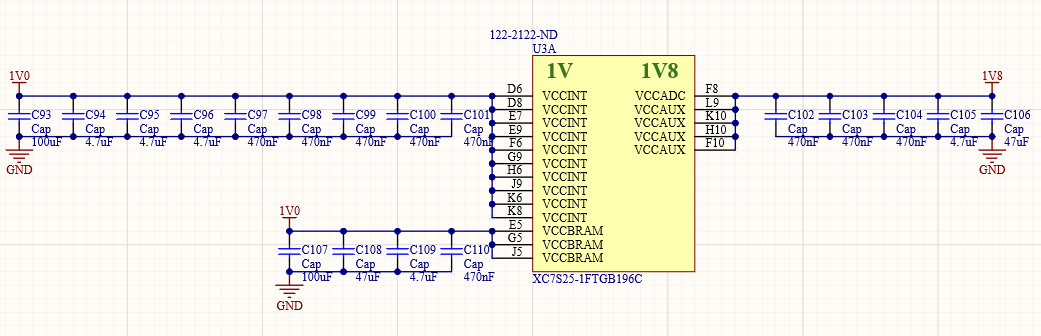
\includegraphics[width=\textwidth]{FPGAPower.PNG}
            \caption{Spartan 7 FPGA Power Supply}
            \label{fig:FPGAPower}
        \end{figure}
            
        The last connections from the LMS are to the Spartan 7 FPGA acting as the baseband modulator. The power supply for the FPGA can be seen in figure \ref{fig:FPGAPower}. All of the decoupling capacitors were chosen based on the specifications given by Xilinx in their datasheet for FPGA power supplies. All capacitors meet or exceed the required ESR and ESL. The FPGA also has a number of grounds which are not pictured.
            
        \begin{figure}[H]
            \centering
            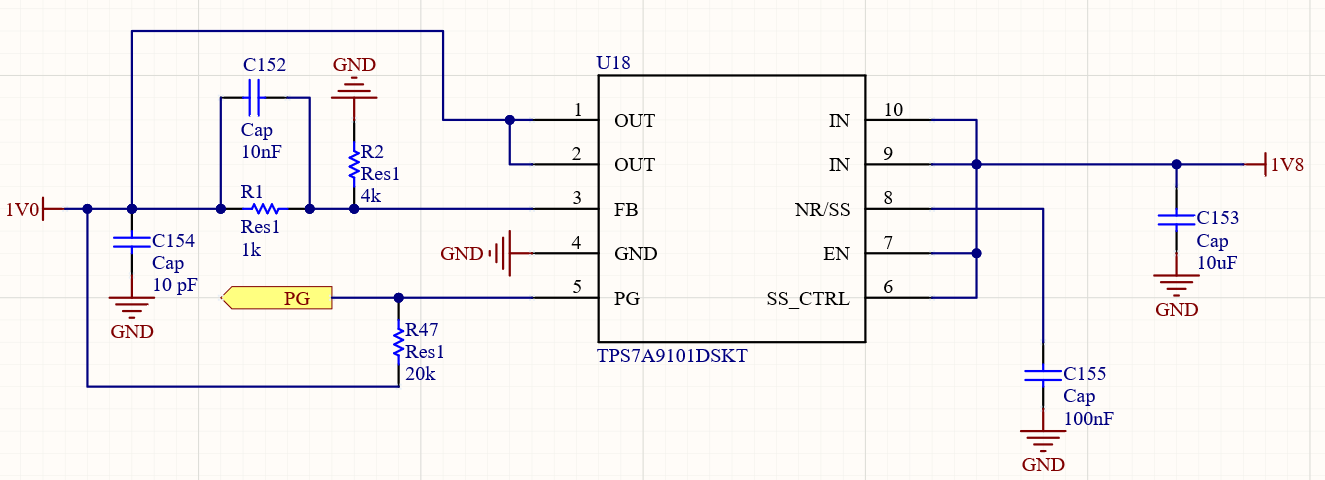
\includegraphics[width=\textwidth]{FPGA1V.PNG}
            \caption{The Linear Regulator Used for the 1V Rail}
            \label{fig:FPGA1V}
        \end{figure}
            
        In order to function, the FPGA also requires a 1V power rail, which is not provided by the PMS. This is generated locally, on the board, by using a linear regulator on the 1.8V power rail, which is shown in figure \ref{fig:FPGA1V}. Using a linear regulator helps to ensure our noise is within the required margins and simplifies design.
            
        \begin{figure}[H]
            \centering
            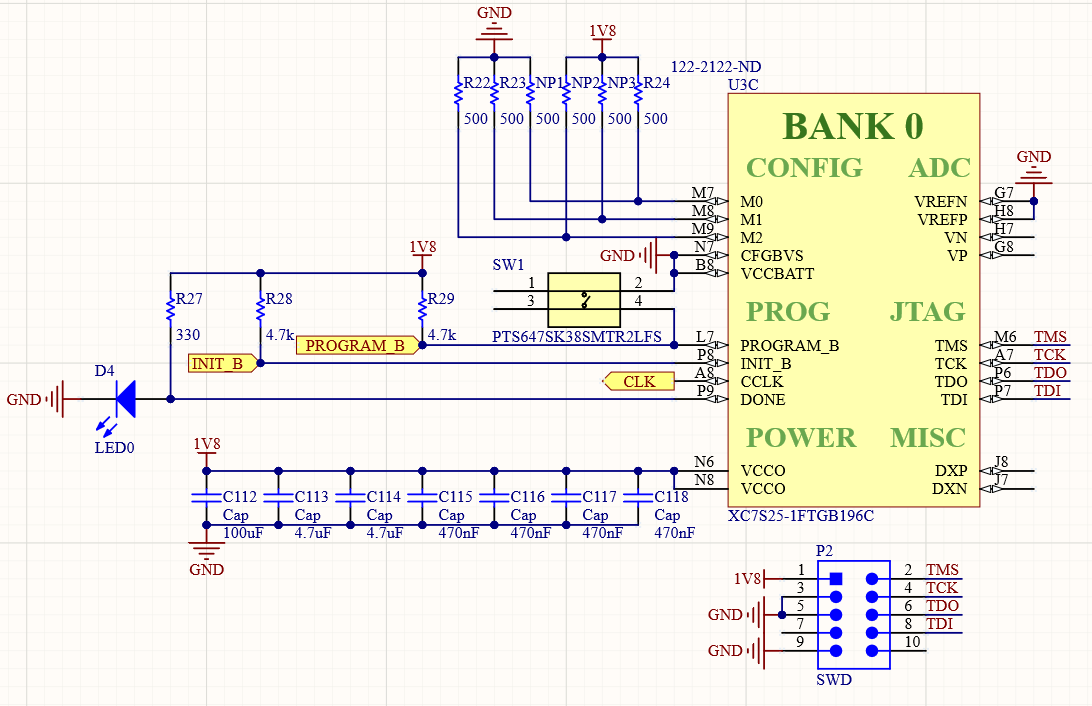
\includegraphics[width=\textwidth]{FPGAConfig.PNG}
            \caption{FPGA Configuration Schematic}
            \label{fig:FPGAConfig}
        \end{figure}
            
        The Spartan 7 FPGAs have a section dedicated to configuring their nonvolatile memory type and the I/O voltage range they can use. The majority of this block can be seen in figure \ref{fig:FPGAConfig}. This FPGA is set up to use SPI flash to boot. This is set by pulling the M0, M1, and M2 pins high or low at startup.
            
        On startup, the program B pin is pulled high, which signals the FPGA to begin reading a bitstream from the associated nonvolatile memory. A pushbutton can be used to pull program B down manually in order to reset the FPGA. However, keeping it held low won't prevent the FPGA from beginning its programming sequence. Holding init B low will stop the FPGA from programming itself from nonvolatile memory once it is reset. The done pin is used as an indicator to display if the FPGA successfully programmed itself.
            
        While there is another subsystem which programs the SPI flash directly, an SWD connector was included anyways. This is so if the other programming method fails the FPGA can still be programmed easily. The only downside is the JTAG programmers for Xilinx FPGAs are not cheap.
            
        \begin{figure}[H]
            \centering
            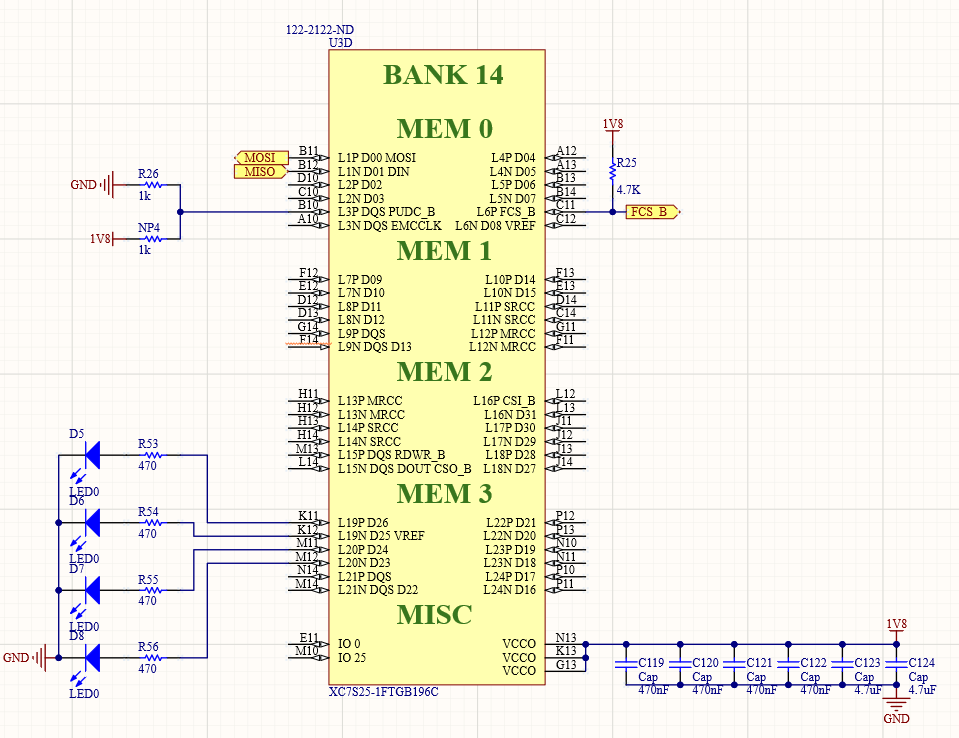
\includegraphics[width=\textwidth]{FPGABank14.PNG}
            \caption{FPGA I/O Bank 14}
            \label{fig:FPGABank14}
        \end{figure}
            
        \begin{wrapfigure}{r}{0.5\textwidth}
            \centering
            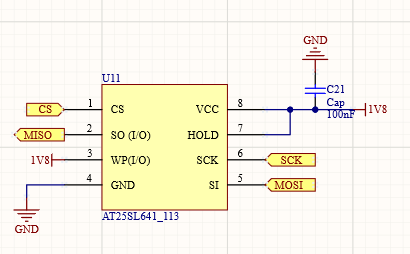
\includegraphics[width=0.48\textwidth]{FPGASPIFlash.PNG}
            \caption{SPI flash used to configure the FPGA}
            \label{fig:FPGASPIFlash}
        \end{wrapfigure}
            
        Figure \ref{fig:FPGABank14} shows the I/O bank that has the final configuration pins for the FPGA. The PUDC B pin determines if the I/O pins will have their internal pull ups enabled or not. The MOSI, DIN, FCS B, and the CLK pin from figure \ref{fig:FPGAConfig} are all used to interface to the SPI flash which can be seen in figure \ref{fig:FPGASPIFlash}.
            
        A group of four LEDs are included on this I/O bank to assist with software testing. Additionally, there are a number of I/O that interact with other subsystems which are not shown. This is because they can be connected to almost any I/O pins on the FPGA, and as a result their exact placement will be determined during PCB routing based on whichever pins make routing the easiest.
            
        \begin{figure}[H]
            \centering
            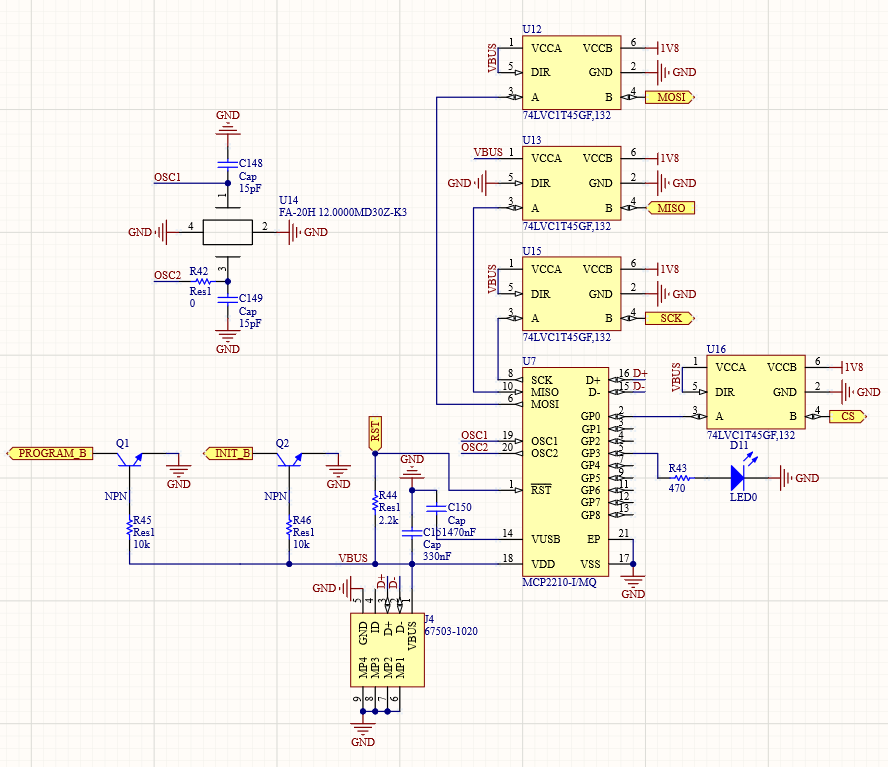
\includegraphics[width=\textwidth]{FPGAUSBSPI.PNG}
            \caption{USB to SPI programming circuit}
            \label{fig:FPGAUSBSPI}
        \end{figure}
           
        Figure \ref{fig:FPGAUSBSPI} shows the circuit used to program the SPI flash over USB. When power is present on the VUSB pin the Program B and Init B pins on the FPGA are both pulled low to put it into reset mode and prevent it from trying to read from the SPI flash while the USB connection is present. From there, the USB data is converted to SPI and level shifters are used to change its voltage to appropriate levels for the SPI flash. From there, the SPI flash can be programmed by sending an appropriately formatted file over the USB connection which contains the SPI flashes write opcode followed by the bitstream data to write to the next address in memory. By doing this, it is possible to program the FPGA directly rather than using JTAG to make the FPGA program the SPI flash.
           
       \begin{figure}[H]
            \centering
            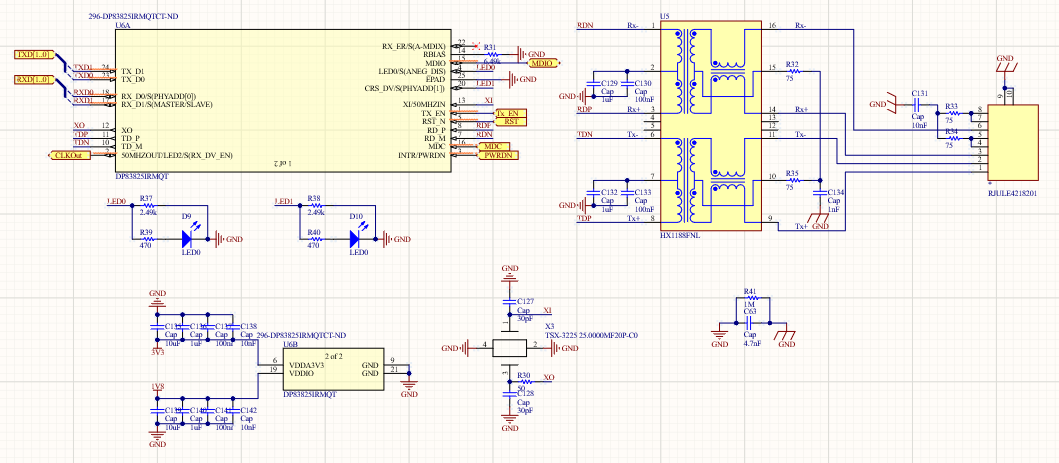
\includegraphics[width=\textwidth]{FPGAEthernet.PNG}
            \caption{Ethernet PHY for the FPGA}
            \label{fig:FPGAEther}
        \end{figure}
        
        The last subsystem that the FPGA connects to is an Ethernet PHY, which is seen in figure \ref{fig:FPGAEther}. This Ethernet setup includes an extremely low profile RJ45 jack in order to fit on the Flight Computer. The RJ45 connector goes straight to a set of isolation transformers which feed into the Ethernet PHY. The RJ45 jack also has its own chassis ground which is connected to the main board ground with a large capacitor and resistor. The Ethernet PHY itself uses RMII to communicate between itself and the FPGA.
      
    \pagebreak   
    \subsubsection{Routing}
        The M2RB is one of the PCBs one the Flight Computer. As a result, it has a standardized shape and mounting holes, as well as keepout areas.
        
        The PCB is four layers in order to improve EMC performance and make 50 Ohm matched traces a reasonable size. These four layers in order from top to bottom are signal, ground, split power, and signal. The split power plane has three distinctive regions which will be discussed in relevant sections.
        
        \begin{figure}[H]
            \centering
            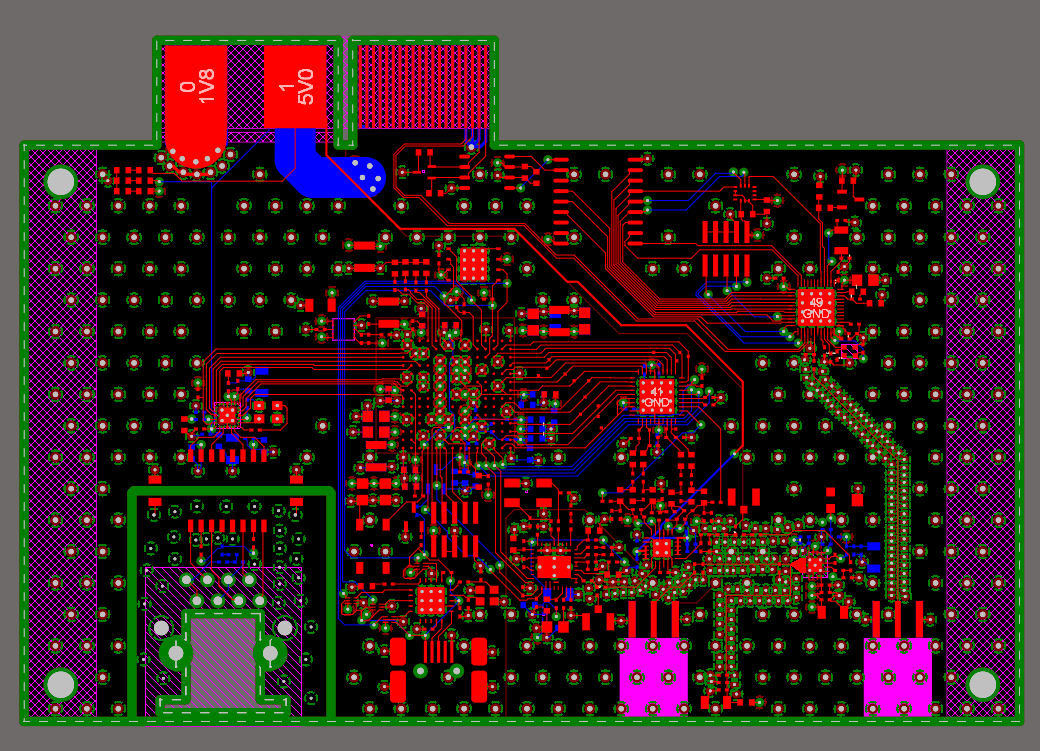
\includegraphics[width=\textwidth]{M2RBPCB.PNG}
            \caption{Fully routed M2RB}
            \label{fig:M2RBPCB}
        \end{figure}
        
        \pagebreak
        
        \begin{figure}[H]
            \centering
            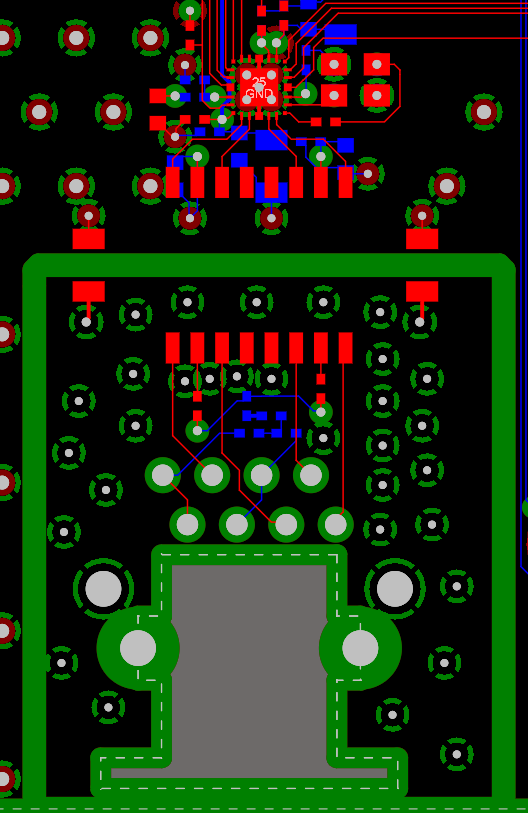
\includegraphics[width=0.65\textwidth,angle = 270]{M2RBEtherRoute.PNG}
            \caption{Ethernet routing}
            \label{fig:M2RBEtherRoute}
        \end{figure}
        
        Figure \ref{fig:M2RBEtherRoute} shows how the Ethernet jack was routed on the M2RB. The large green box shows a split in the ground pours and the planes of the PCB. This was done to isolate the Ethernet ground from the board ground. That helps reduce the chance of ESD events damaging the board and also helps prevent ground loops from generating common mode emissions. The two grounds are tied together with a large resistor and capacitor so that the energy of any ESD events can be dissipated safely.
        
        The differential pairs are kept as close together as possible to prevent any differential mode noise from appearing on them. The isolation transformer is placed with one end on the Ethernet ground and one on the board ground since it is used to change the common mode voltage of the differential pairs to the board ground rather than the Ethernet ground.
        
        In order to avoid transmission line effects, the IC handling Ethernet communication was placed extremely close to the jack. This IC handles communication between the FPGA and Ethernet using RMII.
        
        \pagebreak
        
        \begin{figure}[H]
            \centering
            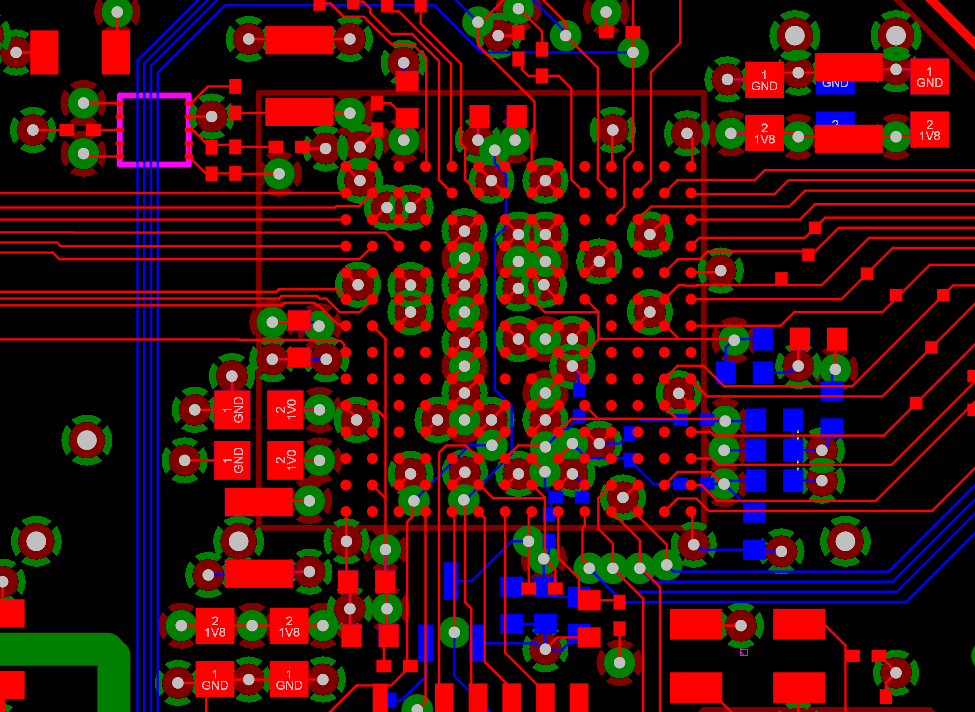
\includegraphics[width=\textwidth]{M2RBFPGARoute.PNG}
            \caption{FPGA routing}
            \label{fig:M2RBFPGARoute}
        \end{figure}
        
        Figure \ref{fig:M2RBFPGARoute} shows the routing for the FPGA. The FPGA uses a 1V power plane on the third layer directly below it, and is surrounded by a 1.8V power plane on that same layer. This is done so that the 1V connections can easily be made with a single via since there are more 1V connections than 1.8V connections. The 1.8V plane is kept as close as possible so that the length of the power traces can be kept short to minimize ESL.
        
        Due to the split in the power plane all I/O that runs over the split is kept on the top layer where there is a continuous ground plane. This prevents impedance discontinuities from radiating or making I/O susceptible to noise.
        
        All of the decoupling capacitors are kept as close to the FPGA as possible. The datasheet specifies the maximum distance each capacitor can be from their respective power pins and this design was checked to ensure it met those minimums.
        
        \pagebreak
        
        \begin{figure}[H]
            \centering
            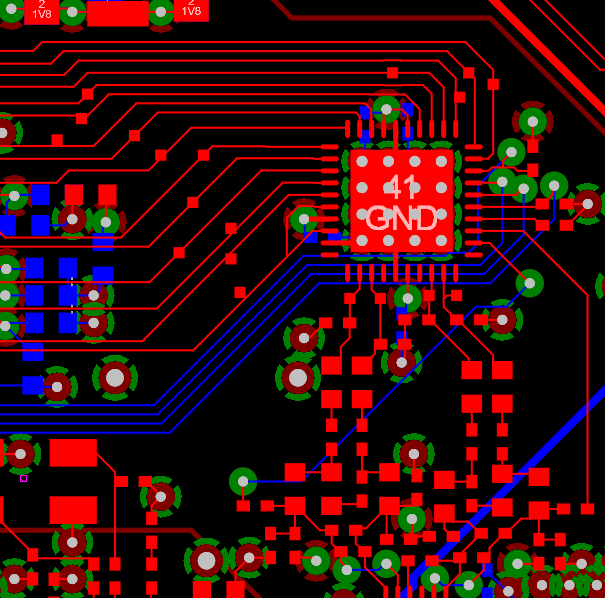
\includegraphics[width=\textwidth]{M2RBDACRoute.PNG}
            \caption{DAC routing}
            \label{fig:M2RBDACRoute}
        \end{figure}
        
        Figure \ref{fig:M2RBDACRoute} shows how the DAC was routed. The majority of the DAC is taken up by the parallel port input from the FPGA. Each of these I/O lines have an exposed pad on them so that they can be easily probed for debugging.
        
        The outputs of the DAC also have a differential filter connected to them. These differential filters are routed to minimize the distance between the differential pairs in order to reduce noise on the output.
        
        \pagebreak
        
        \begin{figure}[H]
            \centering
            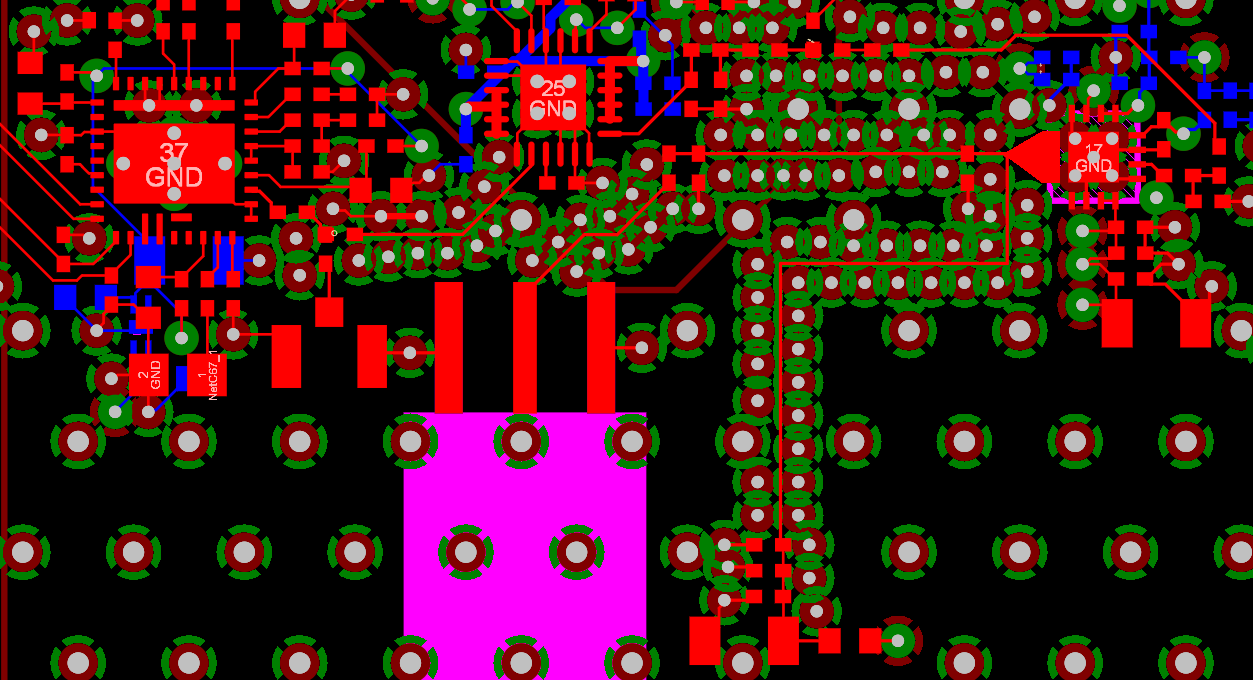
\includegraphics[width=\textwidth]{M2RBModAmpPLLRoute.PNG}
            \caption{RF Section Routing}
            \label{fig:M2RBModAmpPLL}
        \end{figure}
        
        Figure \ref{fig:M2RBModAmpPLL} shows, from left to right, how the PLL, IQ modulator, and power amplifier were routed. The most notable feature is the number of vias. These are included to improve shielding around the RF traces to help reduce unintended emissions.
        
        The other notable feature is the tapered output and long trace on the power amplifier. These were both included by specification of the datasheet. The output is tapered from the full output size down to the size of a 50 Ohm matched transmission line. The long trace connected to the output is a power supply for the amplifier, since it has an open drain output. This follows a very specific shape in order to prevent the RF signal from contaminating the rest of the 3.3V power supply.
        
        The large purple box is where the board will have a cut out to accommodate an SMA connector.
        
        \pagebreak
        
        \begin{figure}[H]
            \centering
            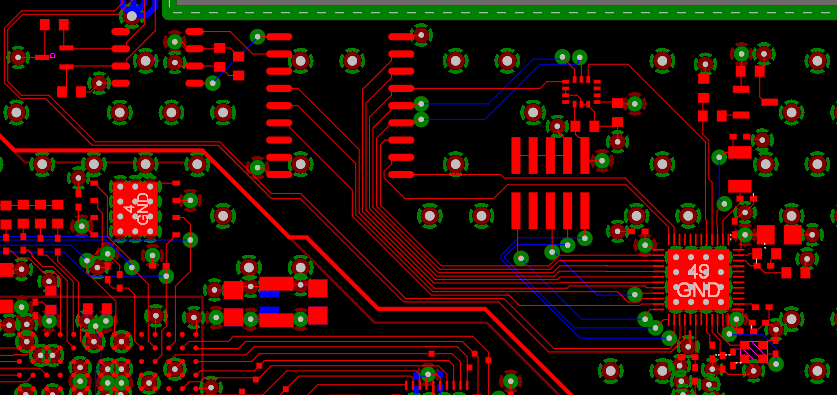
\includegraphics[width=\textwidth]{M2RBnRFRoute.PNG}
            \caption{nRF Routing}
            \label{fig:M2RBnRFRoute}
        \end{figure}
        
        Figure \ref{fig:M2RBnRFRoute} shows how the nRF52832 was routed. This section featured very few restrictions. The only important ones were minimizing the loop size of the internal buck converter and ensuring that the RF output was properly matched and appropriately shielded.
        
        The rest of the picture shows all of the I/O connections of the nRF, mainly to the CAN bus.
        
    \subsubsection{Software}
        \begin{figure}[H]
            \centering
            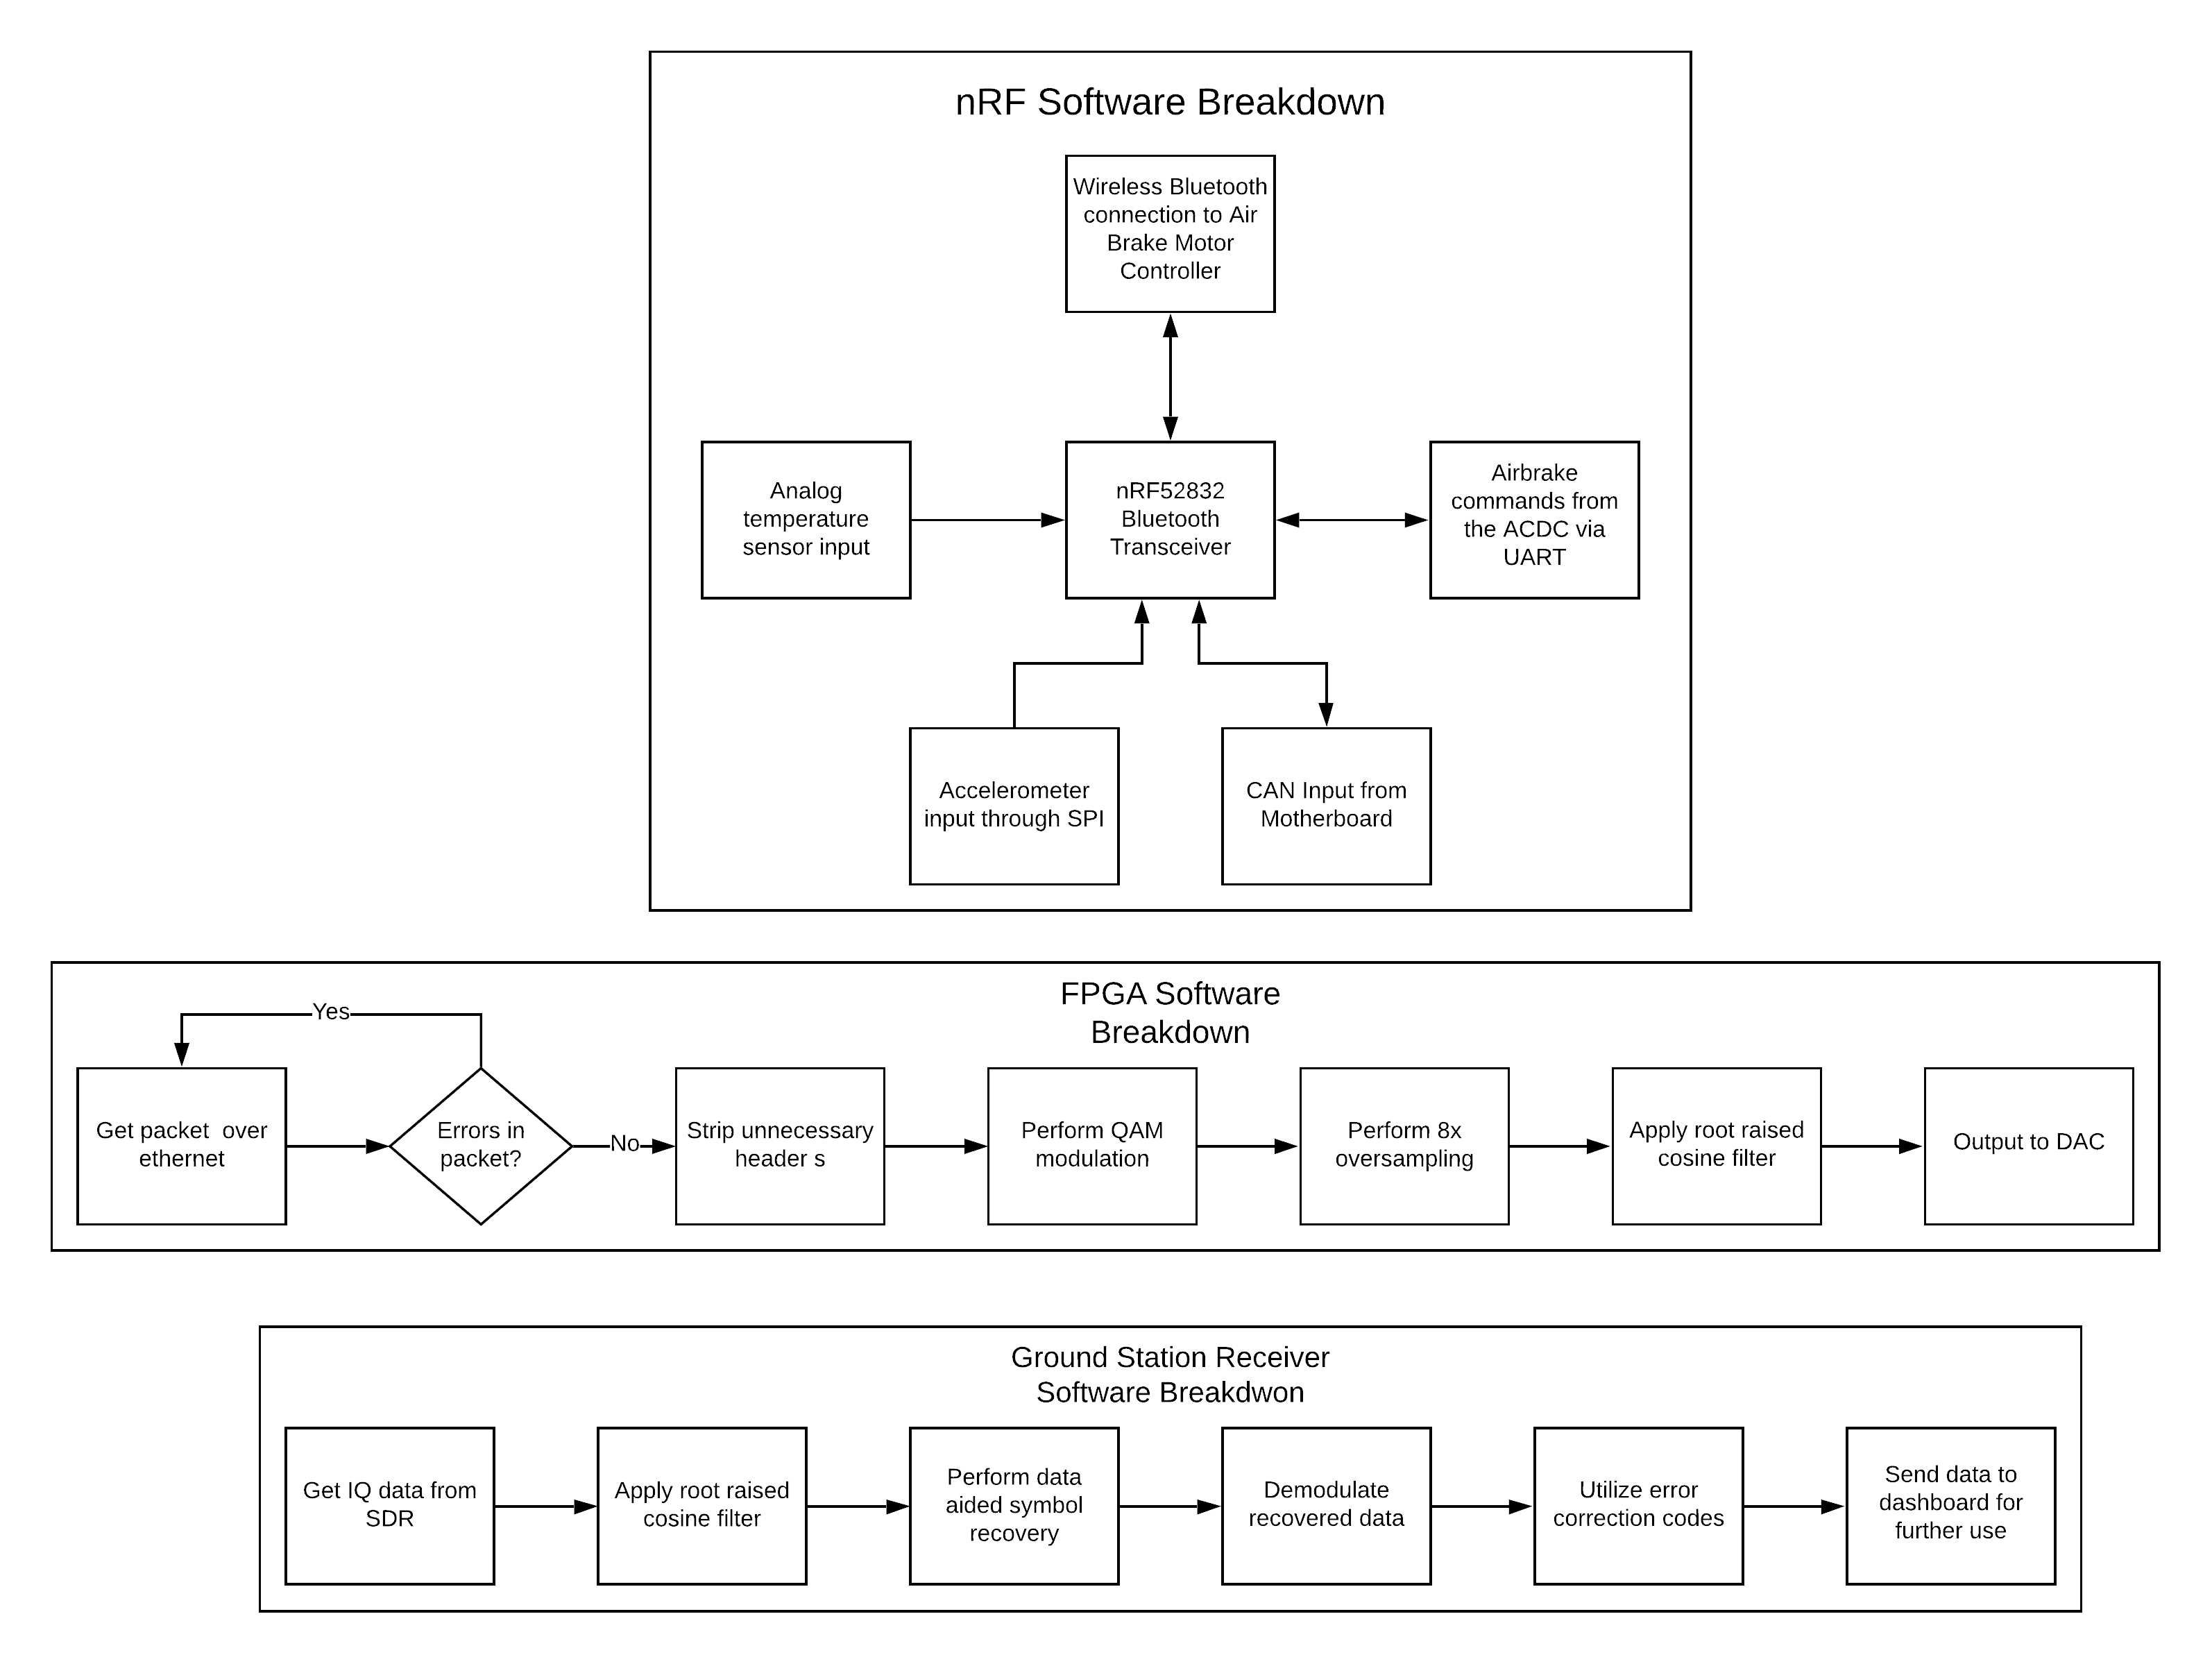
\includegraphics[width=\textwidth]{M2RB Software Breakdown.png}
            \caption{M2RB Software Flowchart}
            \label{fig:M2RBSoftware}
        \end{figure}
            
        The M2RB has three distinct software blocks which are all independent. On the top of figure \ref{fig:M2RBSoftware} the nRF52 software is shown. That software gathers data from the attached sensors and sends it over the CAN bus, and also acts as an intermediary between the ACDC and the ABC.
        
        In the middle of figure \ref{fig:M2RBSoftware} the FPGA software is shown. Data is received with Ethernet. This is handled using a freely available IP core from Xilinx. Once data is received  the FPGA performs error checks to ensure that the data is good, and requests the packet be resent if it detects any errors. Once the packet has been verified good all extra header information that doesn't have to be sent to the ground is removed to reduce the packet size.
        
        From there the outgoing data is modulated with QAM. This can be performed very simply using combinational logic. Once the modulation signal has been generated it will be oversampled eight times. This is simple to do since the signal is essentially a square wave, which means the output is not changing until the input changes. This is done in order to use a root raised cosine filter to band limit the output signal. Once the band limited signal is generated it is then output to the DAC.
        
        On the bottom of figure \ref{fig:M2RBSoftware} the software breakdown for recovering the data at the ground station is shown. IQ samples are initially gathered using an SDR. From there, a root raised cosine filter is applied to complement the root raised cosine filter on the transmitter. From there the symbols need to be recovered from the raw data. In order to do this, Matlab will be used to create a model of the recovery system and then generate the corresponding c++ code. Currently we are planning to use data aided symbol recovery, but depending on performance we may end up using non data aided methods. Once the symbols are successfully recovered they are converted back into binary, and then the data is checked for errors and any error correcting codes included are used to fix the errors. Once the data has been error checked it is sent off to the dashboard for further processing and use.
            
    \subsubsection{Decision Matrix}
        
        Two decisions were made for this system, one for the long ranged solution and one for the short ranged. Table \ref{table:M2RBLongRangeMatrix} shows the long range solution decision matrix. Table \ref{table:M2RBShortRangeMatrix} shows the short range solution decision matrix.
            
        \begin{table}[H]
        \begin{center}
        \begin{tabular}{|c|c|c|c|c|c|c|c|}

        \hline
        System Options & Risk & Difficulty & Benefit & Size & Price & System Engineering & Rating\\ \hline
        Custom Transciever & 1.5 & 4 & 1 & 2 & 5 & 2.5 & 73\% \\ \hline
        Bluetooth & 1.5 & 2.5 & 3 & 2 & 2 & 2.5 & 76\% \\ \hline
        XBee & 1.5 & 1 & 5 & 2 & 2 & 2 & 74\% \\ \hline
        \end{tabular}
        \caption{Long Range M2RB Decision Matrix}
        \label{table:M2RBLongRangeMatrix}
        \end{center}
        \end{table}
            
        \begin{table}[H]
        \begin{center}
        \begin{tabular}{|c|c|c|c|c|c|c|c|}

        \hline
        System Options & Risk & Difficulty & Benefit & Size & Price & System Engineering & Rating\\ \hline
        Bluetooth Mesh & 2.5 & 2 & 2 & 2 & 2 & 2 & 78\% \\ \hline
        ANT & 2.5 & 2 & 2.5 & 2 & 2 & 2 & 76\% \\ \hline
        Zigbee & 2.5 & 2 & 3 & 2 & 2 & 2 & 74\% \\ \hline
        \end{tabular}
        \caption{Short Range Decision Matrix}
        \label{table:M2RBShortRangeMatrix}
        \end{center}
        \end{table}
            
            
         Last year, the long range solution was to use a Bluetooth transmitter. This year's solution is a custom transceiver. It was decided that it would be more optimal even with its increased difficulty and cost. That is because the Bluetooth is not designed for long range. Similarly, the Xbee was not chosen because it would only provide simple telemetry. With the custom transceiver, plans to capture live video to ground are possible, unlike with the Xbee.

        This year, the short range solution is the Bluetooth Mesh standard. Last year, the plan was to use the Adaptive Network Topology. Given that Bluetooth Mesh has faster data rates, use of this system is preferred. Both standards have similar complexity, so slight improvements are expected for the short range solution. Zigbee is another protocol that uses the same band, but it was rejected due to its slower data rates. 
            
    \subsubsection{Timeline}
        
        The M2RB schematic is completed. Routing is currently underway. After routing, purchasing the material for the M2RB will begin. Then, soldering and software development can begin. Development kits and simulations will be used for said software development. After this, testing and optimization will bring the development cycle to a close. The timeline is shown in table \ref{table:M2RBTimeline}.
            
        \begin{table}[ht]
        \begin{center}
        \begin{tabular}{|c|m{2.5cm}|c|c|c|}

        \hline
        Milestone & Description & Start Date & End Date & Duration(Days) \\ \hline
        M2RB Schematic & \raggedright Schematic design for M2RB Board & 6/10/2020 & 10/1/2020 & 113 \\ \hline
        M2RB Board Routing & Route the PCB for the M2RB & 9/15/2020 & 10/20/2020 & 44 \\ \hline
        M2RB Purchasing & \raggedright Order components and PCBs & 11/17/2020 & 12/1/2020 & 14  \\ \hline
        M2RB Soldering & Solder the PCB & 11/24/2020 & 12/19/2020 & 25 \\ \hline
        M2RB Software Core & \raggedright Develop and test software & 12/22/2020 & 2/13/2021 & 53 \\ \hline
        M2RB Final Debugging / Finishing & Refine and optmize code & 3/1/2021 & 6/1/2021 & 92 \\ \hline
        M2RB Simulation / Dev Kit & \raggedright Begin software development via dev kits and simulation & 9/15/2020 & 12/22/2020 & 98 \\ \hline
        \end{tabular}
        \caption{M2RB Timeline}
        \label{table:M2RBTimeline}
        \end{center}
        \end{table}
            
            
    \subsubsection{Work Breakdown Structure}
        
        Table \ref{table:M2RBWBS} shows the M2RB's work breakdown structure.
            
        For the M2RB's research, it is expected to take at most 69 hours and at least 29.25 hours. Thus, there will most likely be an average of 49.125 hours of research. This research consists mainly of component selection. So far, there have been 6 hours of actual research. 

        The M2RB's schematic is expected to take at most 38.1 hours and at least  17.85 hours. This means the M2RB's schematic will most likely taken an average of 27.975 hours. There are 3.5 hours of schematic completed so far. 

        For the M2RB's testing, it will take at most 15.1 hours and at least 7.6 hours. This means there will most likely be an average of 11.35 hours of testing. No testing has been completed for the M2RB yet.

        For the M2RB's programming, it will take at most 79 hours and at least 32 hours. Thus, there will most likely be an average of 55.5 hours of programming. For the debugging and simulation of the M2RB, it will take at most 62 hours and at least 25 hours. The debugging and simulation of the M2RB is expected to average around 43 hours.
            
        
        \begin{landscape}
            \begin{longtable}[c]{|c|m{2cm}|c|m{4cm}|m{2cm}|m{2cm}|m{2cm}|}
            \caption{The Work Breakdown Structure for the M2RB}
            \label{table:M2RBWBS} \\
            
            \hline
            Task & Skill Level & Person & Description & \centering Research (Hr) & \centering Schematic (Hr) & \begin{center} Testing (Hr) \end{center} \\ \hline 
            \raggedright 1V Regulator & \raggedright Beginner to Intermediate & Albi & \raggedright Regulate 1.8V to 1V for the Spartan 7 FPGA & 0.5 & 0.5-1 & 0.25 \\ \hline
            \raggedright CAN Controller & Beginner & Josh & \raggedright Utilize the MCP2515 CAN controller to communicate between the CAN transceiver and MCU/FPGA & 0.5 & 0.5-1 & 0   \\ \hline
            CAN Transciever & Beginner & Josh & \raggedright Utilize the SN65HVD1050D CAN transceiver to communicate between the CAN bus and CAN Controller & 0.5 & 0.5-1 & 0.5-1    \\ \hline
            Ferrite Bead Filters & \raggedright Beginner to Intermediate & Matt & \raggedright Choose ferrite beads that have a high enough DC current capability and a good impedance curve & 0.5-1 & 0.1 & 0.1 \\ \hline
            FPGA Programming Circuit & \raggedright Intermediate to Advanced & Matt & \raggedright Utilize the FT1248 to program the SPI flash via USB to program the FPGA. May be superceded by JTAG programming & 1-3 & 1-3 & 0.5 \\ \hline
            I2C EEPROM & \raggedright Beginner to Intermediate & Erin & \raggedright Implement I2C EEPROM for the LMS7002M MCU to boot from & 2 & 1 & 0  \\ \hline
            LMS7002M & Advanced & Matt & \raggedright Implement the LMS7002M RFIC transceiver & 2-4 & 3-5 & 1-3  \\ \hline
            LMS7002M Rx Filter + Balun & Beginner & Erin & \raggedright Implement the impedance matching filter and balun from the LMS7002M transmitter to the power amplifier & 0.5-1 & 0.5-1 & 0.25 \\ \hline
            LMS7002M Tx Filter + Balun & Beginner & Erin & \raggedright Implement the impedance matching filter and balun from the LMS7002M transmitter to the power amplifier & 0.5-1 & 0.5-1 & 0.25 \\ \hline
            nRF52832 & \raggedright Beginner to Intermediate & Justin & Implement the nRF52832 IC &  1-2 & 1.5-4 & 0.5-2 \\ \hline
            nRF52832 Impedance Matching Filter & Beginner & Justin & \raggedright Implement the impedance matching filter from the nRF52832 to the its antenna & 0.5-1 & 0.5-1 & 0.25 \\ \hline
            Power Amplifier & \raggedright Beginner to Intermediate & Albi & \raggedright Utilize the SKY65111-348LF power amplifier to increase the output power of the LMS7002M & 0.5-1 & 1-3 & 0.5 \\ \hline
            Spartan 7 FPGA & Advanced & Matt & \raggedright Implement the XC7S25 FPGA to act as the baseband modulator & 2-4 & 3-5 & 1-3 \\ \hline
            SPI Flash & \raggedright Beginner to Intermediate & Albi & \raggedright Implement SPI flash for the FPGA to boot from & 0.5 & 0.5-1 & 0 \\ \hline
            Temp Sensor & Beginner & Justin & \raggedright Implement the LM50 temp sensor & 0.25-0.5 & 0.25-1 & 0.25   \\ \hline
            Ethernet to FPGA Interface & \raggedright Intermediate to Advanced & Matt & \raggedright Utilize the DP83825IRMQT to interface Ethernet to the FPGA using RMII & 1-3 & 1-3 & 0.5 \\ \hline
           LMS7002M Clock & \raggedright Intermediate & Matt & \raggedright Set up a high accuracy clock to feed the LMS7002Ms PLLs & 1-2 & 1-2 & 0.5 \\ \hline
            Vibration sensor and Accelerometer & Beginner & Justin & \raggedright Integrate vibration sensor into circuit board & 0.5-1 & 1 & 1 \\
            \hline
            \end{longtable}
            
        \end{landscape}
        
            

\end{document}

